\documentclass[a4paper,12pt]{article}
\usepackage[utf8]{inputenc}
\usepackage[english]{babel}
\usepackage{fancyhdr}
\usepackage{float}
\usepackage{hyperref}

%Use this to customize margins
\usepackage[
  top=2cm,
  bottom=2cm,
  left=1cm,
  right=1cm,
  headheight=17pt, % as per the warning by fancyhdr
  includehead,includefoot,
  heightrounded, % to avoid spurious underfull messages
]{geometry} 

%Use this to customize headers
\pagestyle{fancy}
\fancyhf{}
\fancyhead[LE,RO]{Report version: \today}
\fancyhead[RE,LO]{ReMeltRadar 2021/22}
\fancyfoot[CE,CO]{\leftmark}
\fancyfoot[LE,RO]{\thepage}
\usepackage{graphicx}
\renewcommand{\headrulewidth}{2pt}
\renewcommand{\footrulewidth}{1pt}


\usepackage{blindtext}

%Use this to customize tables
\usepackage[table]{xcolor}
\setlength{\arrayrulewidth}{1mm}
\setlength{\tabcolsep}{18pt}
\renewcommand{\arraystretch}{1.5}
\linespread{1.25} % also use linespacing > 1? JH 2022-03-21
%\arrayrulecolor[HTML]{fffff}

%Use this to customize colors
\definecolor{babyblueeyes}{rgb}{0.63, 0.79, 0.95}
\definecolor{beaublue}{rgb}{0.74, 0.83, 0.9}
\definecolor{bluegray}{rgb}{0.4, 0.6, 0.8}

%Here some pre-defined commands
\newcommand{\ProtocolTable}[6]
{
\begin{table}[]
\begin{tabular}{|p{1.8cm} p{3.8cm} p{1.8cm} p{2.0cm}|}
\hline
 \rowcolor{beaublue}\textbf{Name}:&\multicolumn{3}{l}{#1} Note \\
 \rowcolor{beaublue}\textbf{Folder:}&\multicolumn{3}{l}{#2} Note \\
 \rowcolor{beaublue}\textbf{Instrument:}&#3&\textbf{Date:}&#4 Note \\
  \rowcolor{beaublue}\textbf{Operator:}&#5&\textbf{Location:}&#6\\
\hline
\end{tabular}
\end{table}
}

% JH Added Packages
\usepackage[bottom]{footmisc}
\usepackage{siunitx}
\usepackage[outline]{contour}
\usepackage{tikz}
\usetikzlibrary{positioning,calc}
\usepackage{circuitikz}
\usepackage{url}
\usepackage{longtable}

\definecolor{ucl_red}{HTML}{D50032}
\definecolor{UCLdarkblue}{HTML}{003D4C}

% Define ApRESDOC command to show details of ApRES profiles
\newcommand{\apresdoc}[9]{
    \def\tempapfname{#1}
    \def\tempaploc{#2}
    \def\tempapcom{#3}
    \def\temptimestamp{#4}
    \def\tempafgain{#5}
    \def\temprfattn{#6}
    \def\tempperiod{#7}
    \def\tempflow{#8}
    \def\tempfupp{#9}
    \apresdoccont
}
\newcommand{\apresdoccont}[6]{
  \def\tempnatt{#1}
  \def\tempnchirp{#2}
  \def\tempnsubburst{#3}
  \def\temppowercode{#4}
  \def\tempbattvolt{#5}
  \def\tempaplbl{#6}

  \begin{table}
    \caption{\tempapcom}
    \rowcolors{2}{gray!25}{white}
    \centering
    \includegraphics[width=0.9\textwidth]{Figures/ApRES/Rover/HF/\tempapfname.png}
    \\
    ~\\
    \begin{tabular}{>{\bfseries}l l >{\bfseries}l l}
      \hline
      \rowcolor{gray!50}
      \multicolumn{4}{c}{\textbf{Filename} \tempapfname} \\
      \hline
      Param. & \bfseries Value & Param. & \bfseries Value \\
      AF Gain & \tempafgain &
      RF Attn. & \temprfattn \\
      Subbursts & \tempnsubburst &
      Period ($T$) & \tempperiod~s \\
      Bandwidth & \tempflow~-~\tempfupp~MHz &
      Power Code & \temppowercode \\
      Batt. Volt. & \tempbattvolt~V &
      - & - \\
      \hline
    \end{tabular}
    \label{\tempaplbl}
  \end{table}
}

%Start the document here.

\begin{document}
\section{Summary of ReMeltRadar 2021/22}
\begin{figure}
  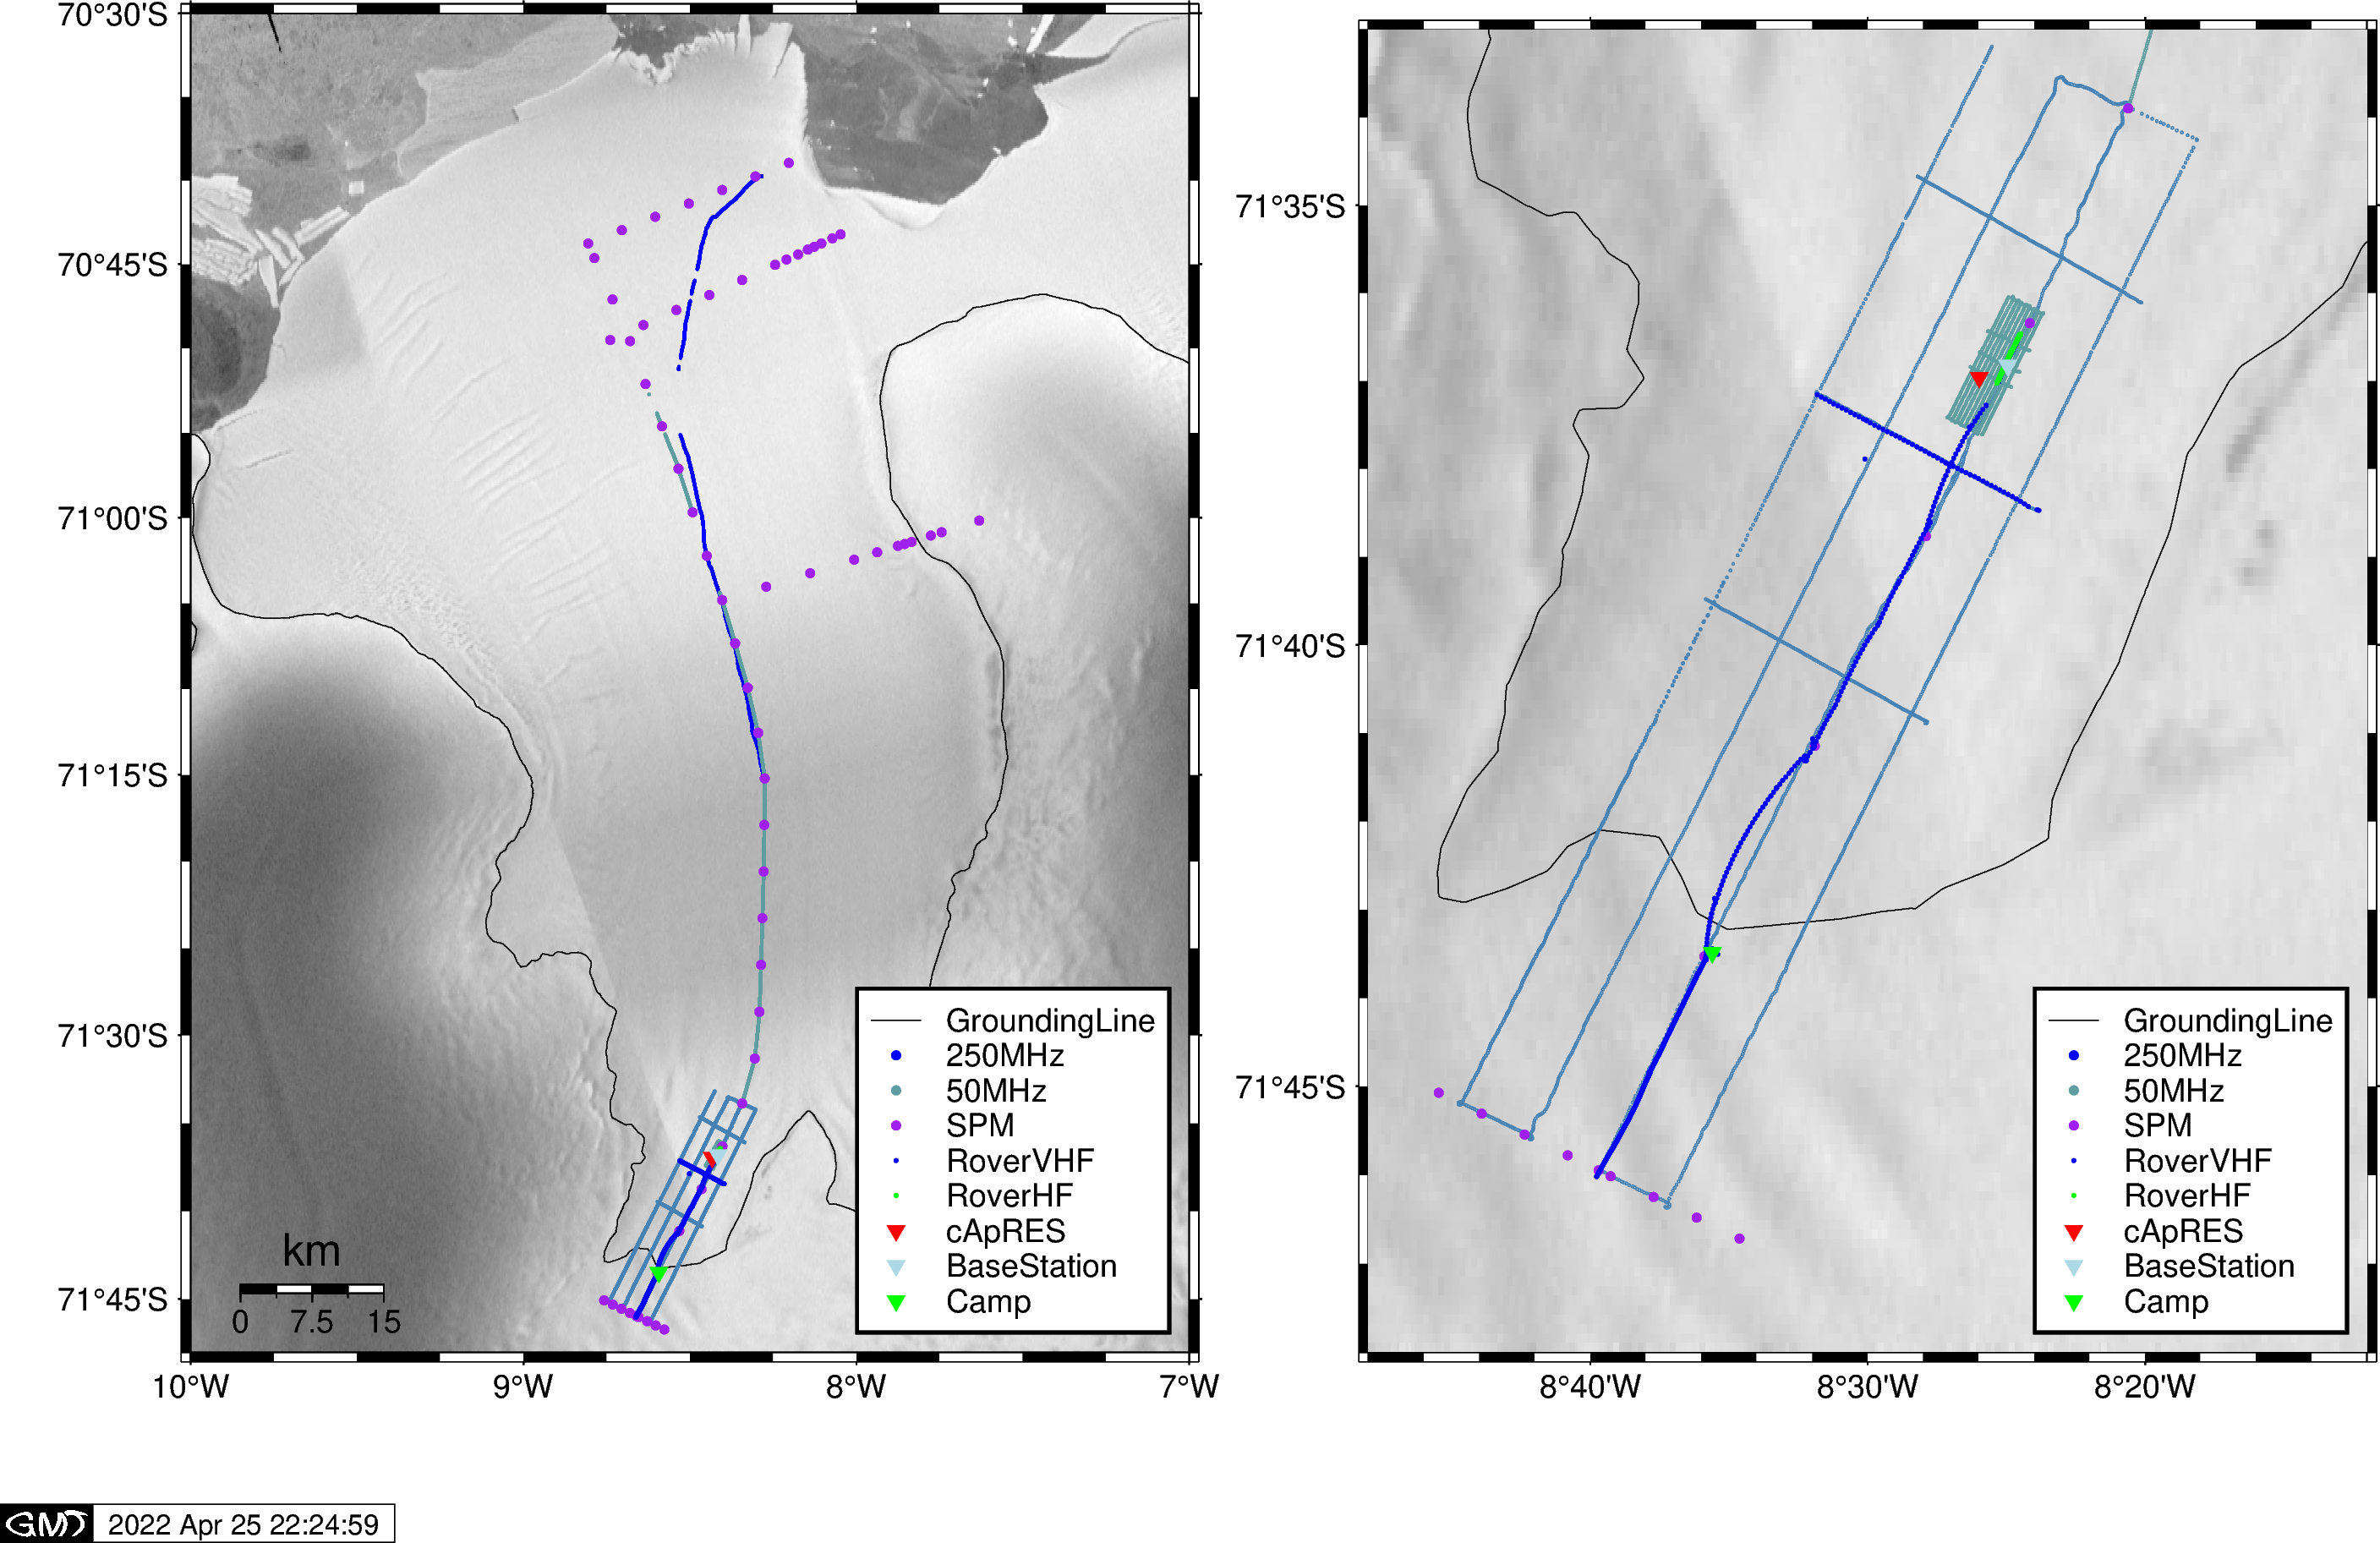
\includegraphics[width=\linewidth]{Figures/Overview.png}
  \caption{(Left) Larger-scale bird's eyes perspective of 250 MHz GPR, 50 MHz GPR, static \& polarimetric (SPM) and continuous ApRES (cApRES) locations at Ekström Ice Shelf, East Antarctica. (Right) Close-up of the survey grid close to the grounding-zone.}
  \label{fig:overview}
\end{figure}
\subsection{Objectives}
Ocean induced melting at the bottom of Antarctic ice shelves accounts for approximately half of the total ice-mass loss of the Antarctic Ice Sheet. However, processes that govern the heat exchange at the ice-ocean interface are notoriously difficult to observe. Consequently, the coupling between ice- and ocean models rely on a number of poorly constrained parametrizations which require more observational support both spatially and temporally. Moreover, ice-shelves decelerate the ice discharge from tributary glaciers, and the magnitude of deceleration depends on the mechanical rigidity of the ice shelf itself. This rigidity is governed by a non-newtonian, temperature dependent and anisotropic ice-shelf rheology. This also requires observations as model calibration model calibration to todays ice thickness or velocities is strongly underconstrained.
ReMeltRadar's objectives are (1) to quantify the spatial variable ocean-induced melting from seasonal to centennial timescales, (2) understanding processes that govern ocean-induced melting at sub-kilometers scales, and (3) to map spatial variability in ice anisotropy across different flow regimes. We aim to achieve these objectives with a combination of methods that include model-data fusion (i.e., inversion of the radar stratigraphy using ice-flow forward models), instrument development (i.e., a novel radar combined with an autonomous rover), and profiling with radar polarimetry that is sensitive to the crystal lattice structure.
\subsection{Field work}
The area of interest is the Ekström Ice Shelf, East Antarctica, using the Neumayer station as a logistical hub for field surveys on the ice shelf and in the grounding zone. The first field season took place from 11/2021 – 01/2022. Repeat measurements are planned for the successive field season in 2022/23. 
Field work was conducted in parts using Skidoos and the Hiluxes operating directly from Neumayer station. In a second phase, data were collected after a 120 km traverse with snow tractors from Neumayer to the southern grounding line of the Ekström Ice Shelf (Fig. 1). Logistics were efficiently shared with the GrouZe Project operating in the same area.

%% ******************************************************
%% ******************************************************
\pagebreak
%% ******************************************************
%% ******************************************************
\subsection{Team composition and chronology of data collection}
\begin{table}
\rowcolors{2}{gray!25}{white}
\begin{tabular}{llll}
  \rowcolor{gray!50}
  Name & Project& Deployment& Responsibility\\
  \hline
Reinhard Drews (UT) & ReMeltRadar  &27.12.21-13.12.22& Science Coordination\\  
Inka Koch (UT) & ReMeltRadar & 27.12.21-13.12.22& PulseEkko GPR\\
Jonathan Hawkins (UCL) & ReMeltRadar  &27.12.21-13.12.22& HF ApRES\\
Reza Ershadi (UT) & ReMeltRadar &05.11.21-13.12.22& Rover, SPM\\
Olaf Eisen (AWI) & ReMeltRadar  &05.11.21-13.12.22& Traverse Leader\\
  \hline
\end{tabular}
\caption{\label{TableGPR}Team composition of ReMeltRadar with members of University of Tübingen (UT), University College London (UCL), and Alfred Wegener Institute (AWI).}
\end{table}
%% ******************************************************
%% ******************************************************
\section{Data structure and initial source codes}
\textbf{RD, JH}
%% ******************************************************
%% ******************************************************
\pagebreak
%% ******************************************************
%% ******************************************************
\section{GPR: Data example, field picture, system setup and profile specifics}
\label{SecGpr}
\textbf{This section was written by Inka Koch}
(\href{mailto:inka.koch@uni-tuebingen.de}{\color{blue}{Email Me}})\\

Ground penetrating radar data was collected with the Pulse Ekko System primarily using unshielded antennaes with frequencies of 50 (100) MHz (Table \ref{Table_PE}). A shielded antennae of 250 MHz was only employed once on the traverse to the grounding line (Table \ref{Table_PE}). For the unshielded anteannae the radar transmitter and receiver were set up on a Nansen sled whereas the GPS was set up on the back of the skidoo (Fig. \ref{fig_PE}). This setup of the GPS on the skidoo was determined by the length of the cable from the control unit, which needed to be operated by a person sitting on the back of the skidoo. The system needed to be triggered manually due to a limitation with the system software that did not allow free run data collections for time windows > 2000 ns (*note: the system software update should be ready and tested mid 2022*). More than 100 km of data were collected with 50 MHz by skidoo driving at ca. 10 km per hour triggering the radar manually approximately every second (Fig. \ref{fig:overview}). This allowed imaging of the ice shelf base up to depths of approximately 1000 m close to the ice shelf grounding line (Fig. \ref{fig_PE_bulge}) and detailed imaging of internal ice shelf structures close to the ice shelf surface (Fig. \ref{fig_IRH1}). The Pulse Ekko was hence the diagnostic tool with which a location with steep side walls (henceforth called 'the buldge' as in Fig. \ref{fig_PE_bulge}) could be selected. This section was subsequently surveyed by the rover and a HF ApRES radar (see Section \ref{SecHFApRES}). In addition a fine grid was surveyed close to the location of the bulge  (Fig. \ref{fig:overview}). Hereby a location with basal steps was selected (Fig. \ref{fig_PE_ApRES_site}) where an ApRES was installed for overwintering. The 50 MHz radar data does not only show the base of the ice shelf, internal layers have also been imaged in the top ca. 200 m of the ice shelf (Fig. \ref{fig_IRH1} and Fig. \ref{fig_IRH2}). Hereby some unusal cross-cutting structures have been detected in the near-surface (Fig. \ref{fig_IRH2}).  

\begin{figure}[H]
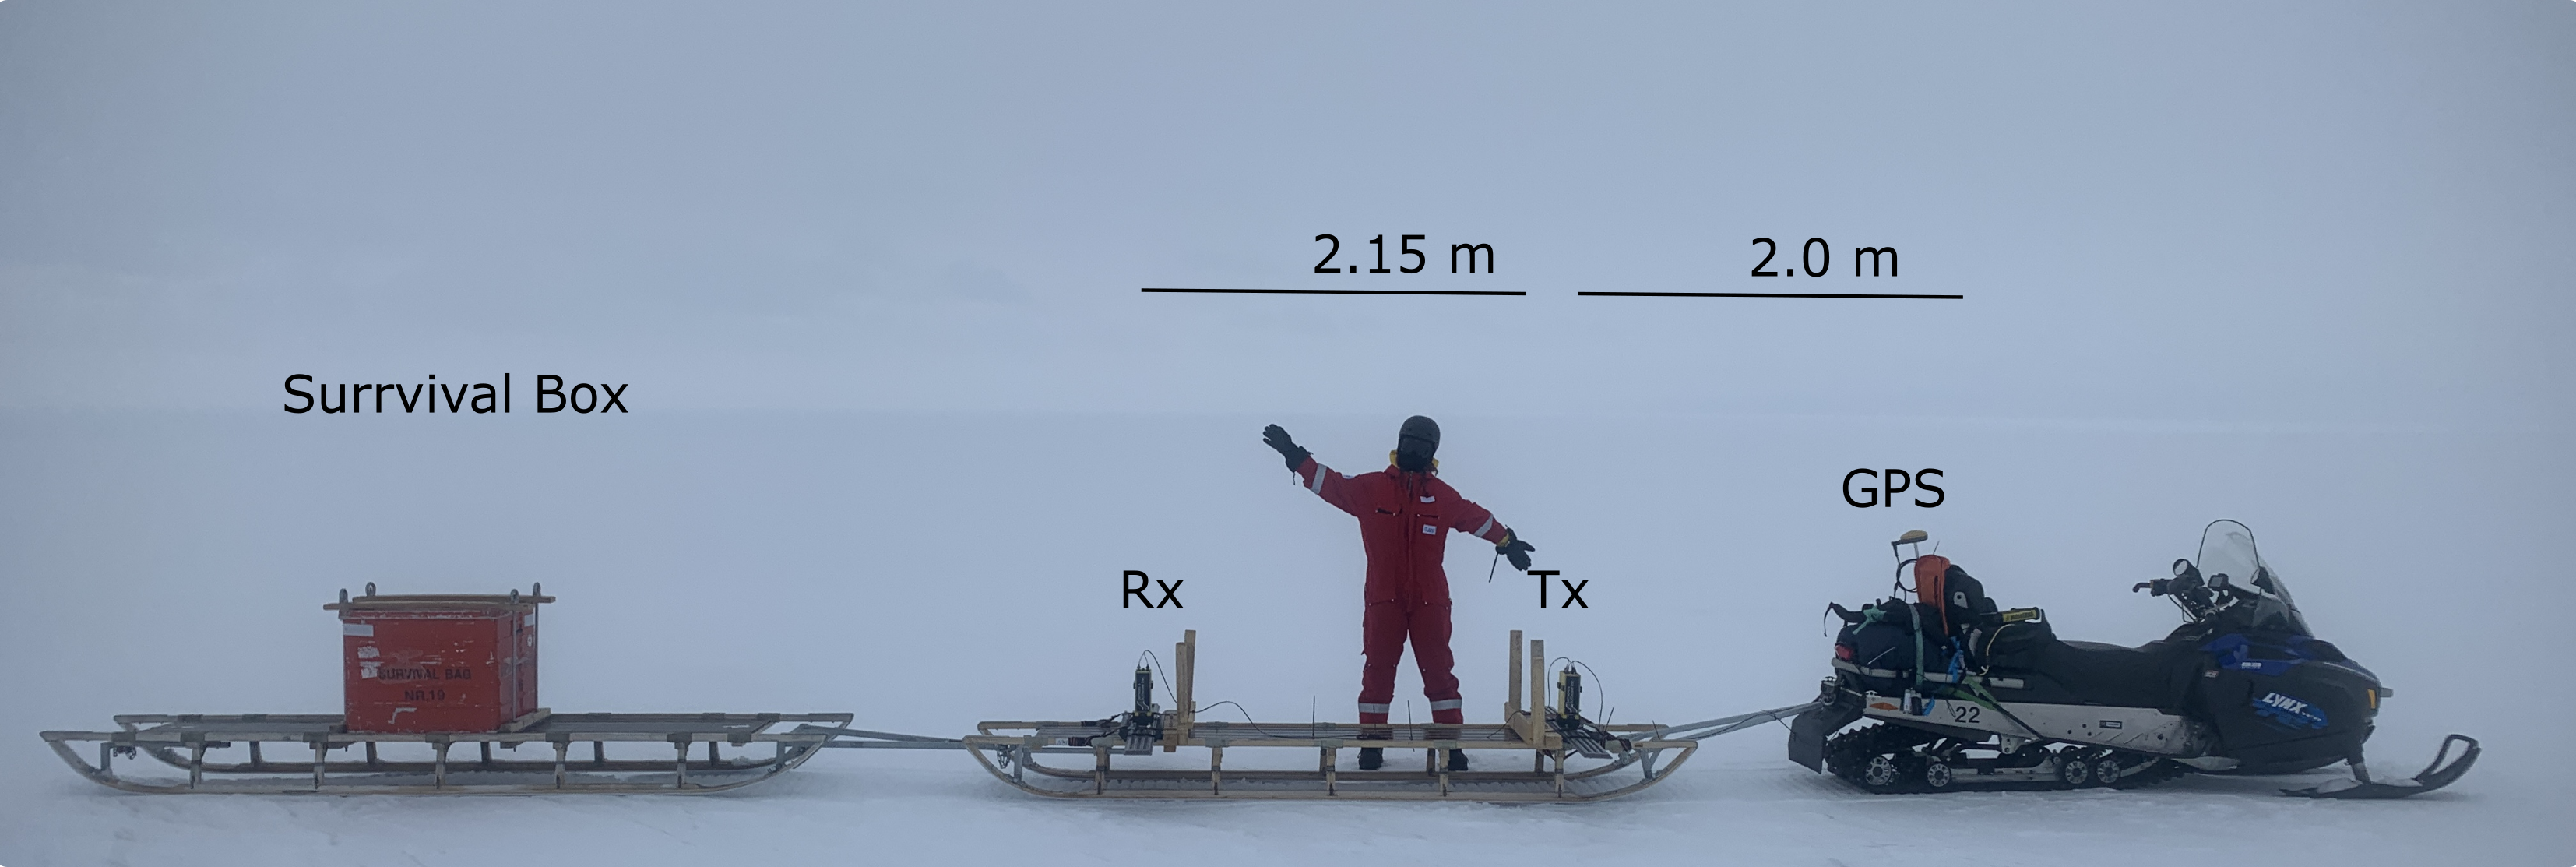
\includegraphics[width=\textwidth]{Figures/PulseEkko/RadarSetup.png}
\caption{Pulse Ekko System setup}
\label{fig_PE}
\end{figure}
\begin{table}[H]
  \tiny
  \rowcolors{2}{gray!25}{white}
\begin{tabular}{m{1cm} m{1 cm} m{5cm} m{7cm}}
    \rowcolor{gray!50}
    Date & Frequency & Profile & File-ID\\
    \hline
    28.12.21 & 50, 100 MHz & Test profiles near NM& \textit{NMIII1.gpz, NMIII100.gpz, NM250Mhz.gpz}\\
    29.12.21 & 100 MHz & MPA01-MPA03, SPX4-SPX2 near NM& \textit{20211229 100MHz Meltprofile.gpz}\\
    01.01.22 & 250 MHz  & NM-SPMA25 during traverse& \textit{Kotta1 250MHz central flow.gpz, Kotta2 250MHz central flow.gpz}\\
    02.01.22 & 50 MHz & GZ profiling along flow (SPMA25-SPMA21-GLPE3n-GLPE4s)& \textit{GL FL 50 MHz 1.gpz}\\
    03.01.22 & 50 MHz & GZ profiling along flow (GLPE4s-GLPE1s-GLPE2n transfer to SPMA25)& \textit{GL FL 50 MHz along 2.gpz, GL FL 50 MHz along 3.gpz, GL FL 50 MHz along 4.gpz}\\
    04.01.22 & 50 MHz & GZ profiling along flow (GLPE7n-GLPE8s-GLPE5s)& \textit{20220104 GL FL 50 MHz along 5.gpz, 20220104 GL FL 50 MHz along 6.gpz, 20220104 GL FL 50 MHz along 7.gpz}\\
    05.01.22 & 50 MHz & GZ profiling across flow & \textit{20220105 GL FL 50 MHz across 12.gpz, 20220105 GL FL 50 MHz across 345.gpz}\\
    06.01.22 & 50 MHz & Finegrid along flow & \textit{20220106 FG EIS 1.gpz, 20220106 FG EIS 2.gpz}\\
    08.01.22 & 50 MHz & Finegrid across flow and some redo around SPM23 & \textit{20220108 FG across EIS.gpz, 20220108 50MHz aroundSPM23.gpz}\\
    10.01.22 & 50 MHz & Along-flow Camp-NM (SPMA21-SPMA10)& \textit{20220110 50MHz along flow long1.gpz, 20220110 50MHz along flow long merged.gpz, 20220110 50MHz along flow long2.gpz, 20220110 50MHz along flow long3.gpz}\\
    12.01.22 & 50 MHz & Camp-NM continuation (SPMA10 - patchy end)& \textit{20220110 50MHz along flow long4.gpz, 20220112 50MHz along flow long5.gpz}\\
    \hline
  \end{tabular}
  \caption{\label{TableGPR}Overview of GPR measurements taken with the PulseEkko radar from Sensors\&Software. Details for the system setup and individual profiles are found in Section \ref{SecGpr}. Operators: I. Koch and R. Drews.}
  \label{Table_PE}
\end{table}
%% ******************************************************
%% ******************************************************
\begin{figure}[H]
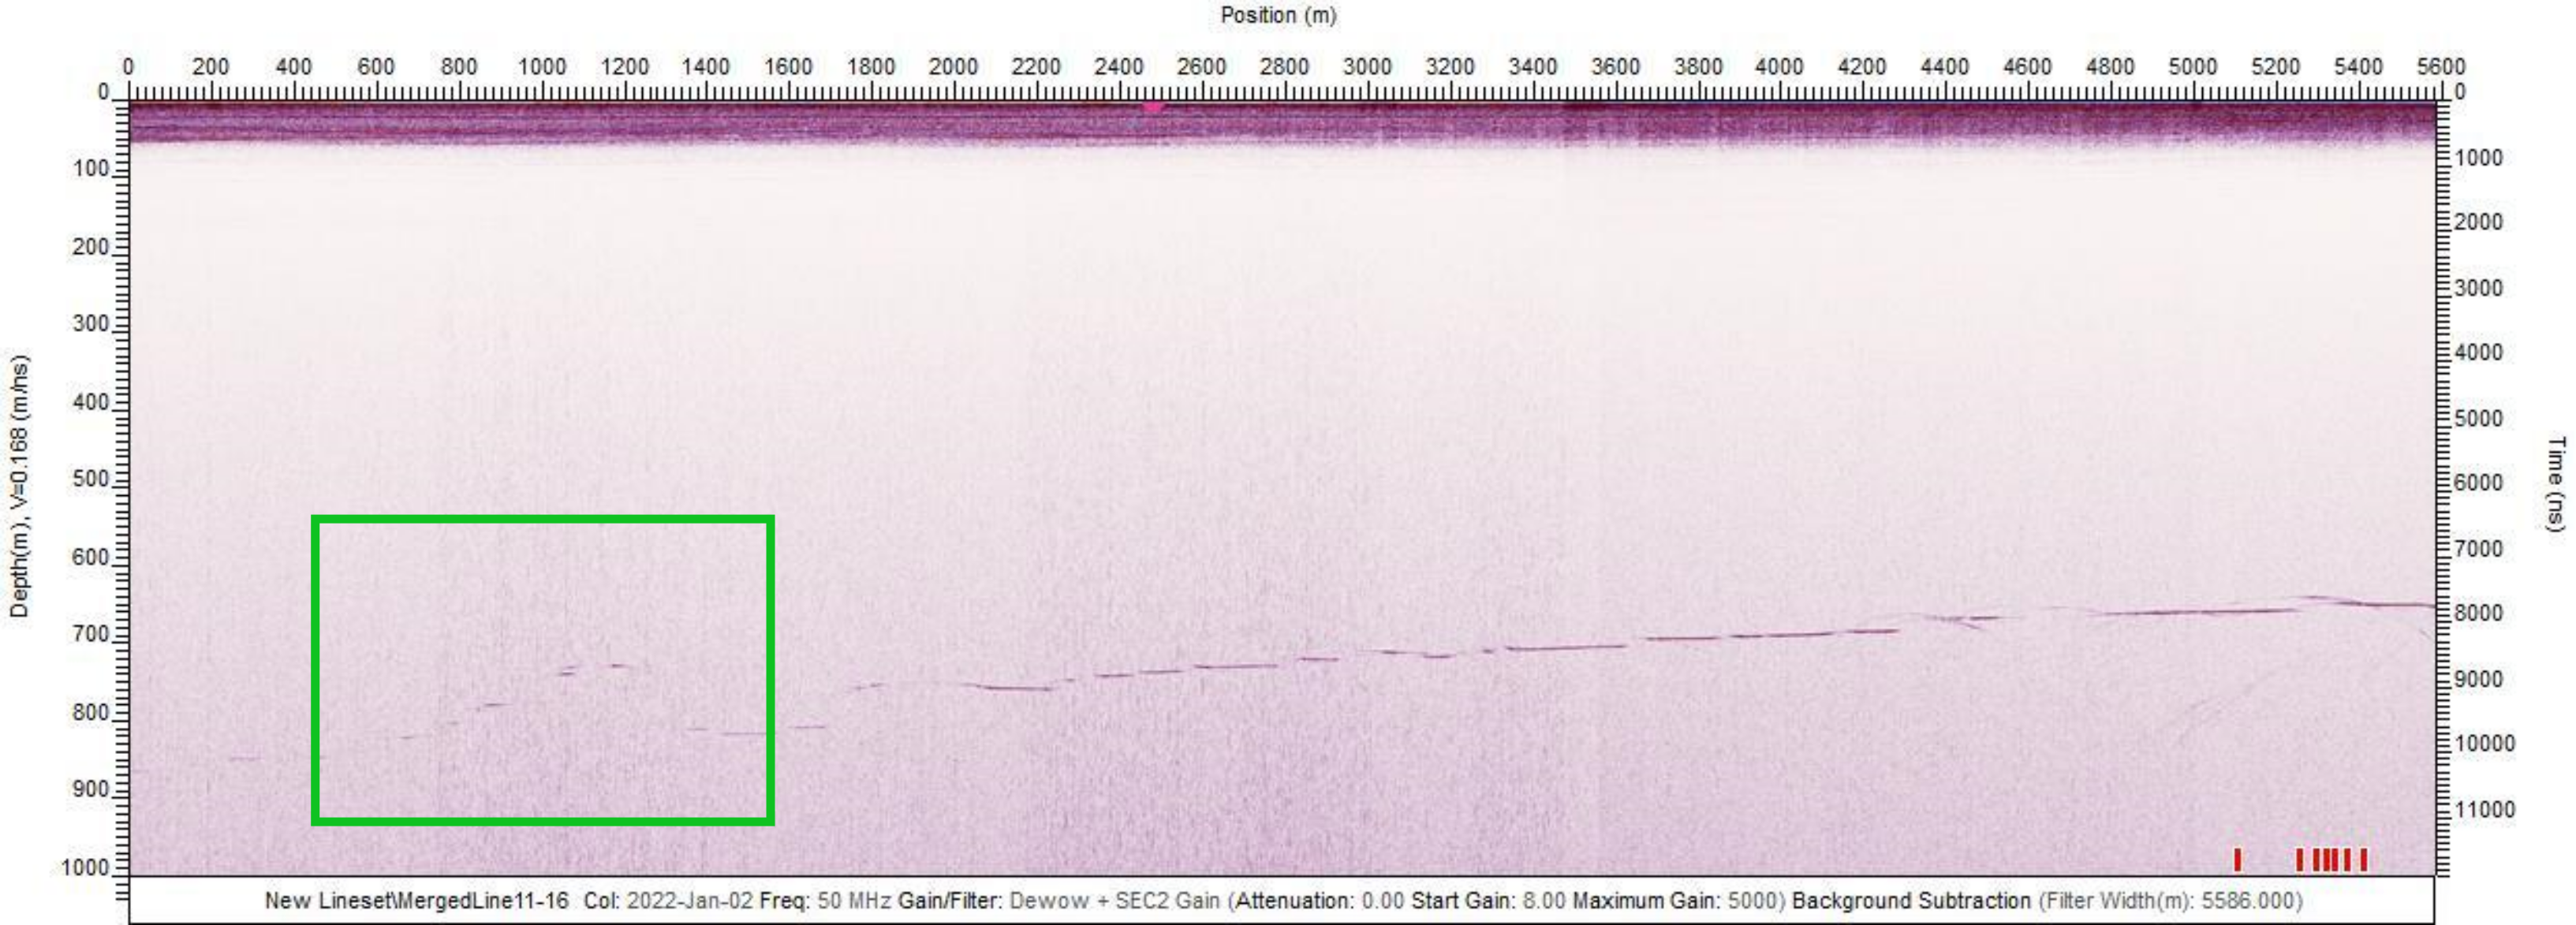
\includegraphics[width=\textwidth]{Figures/PulseEkko/PE_bulge.png}
\caption{Ice shelf base detected with 50 MHz antennae (merged lines 11-16). The location of 'the buldge' is denoted by a green square.}
\label{fig_PE_bulge}
\end{figure}
\begin{figure}[H]
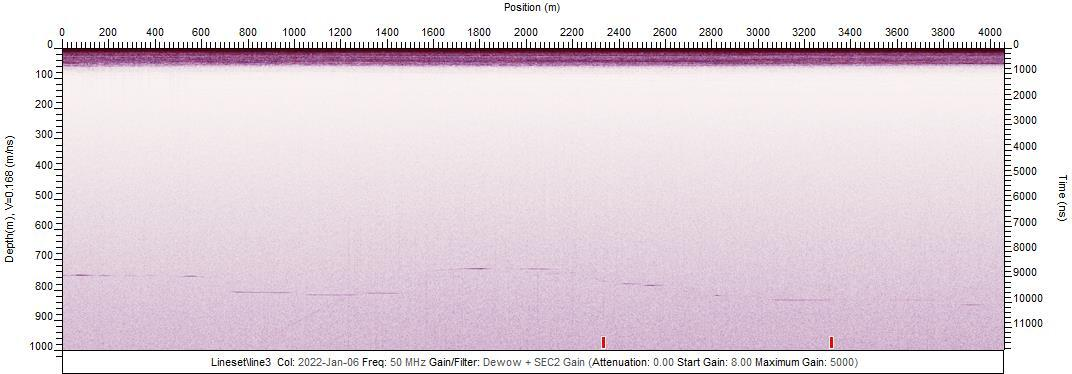
\includegraphics[width=\textwidth]{Figures/PulseEkko/Pulse_Ekko_FG1_line3.jpg}
\caption{Ice shelf base at ApRES site (detected with 50 MHz antennae). Part of the fine grid survey (line 3) as visible in Fig. \ref{fig:overview}.}
\label{fig_PE_ApRES_site}
\end{figure}
\begin{figure}[H]
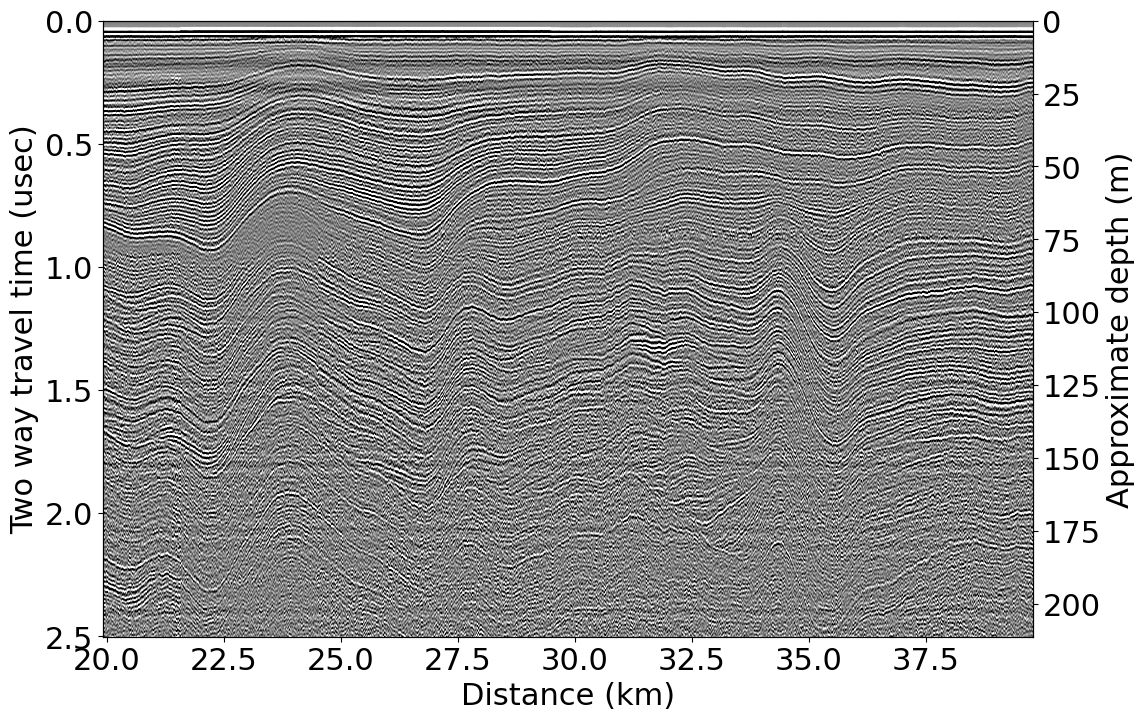
\includegraphics[width=\textwidth]{Figures/PulseEkko/PE_layers_surface.png}
\caption{Internal reflection horizons close to the ice shelf surface (measured with a 50 MHz antennae).}
\label{fig_IRH1}
\end{figure}
\begin{figure}[H]
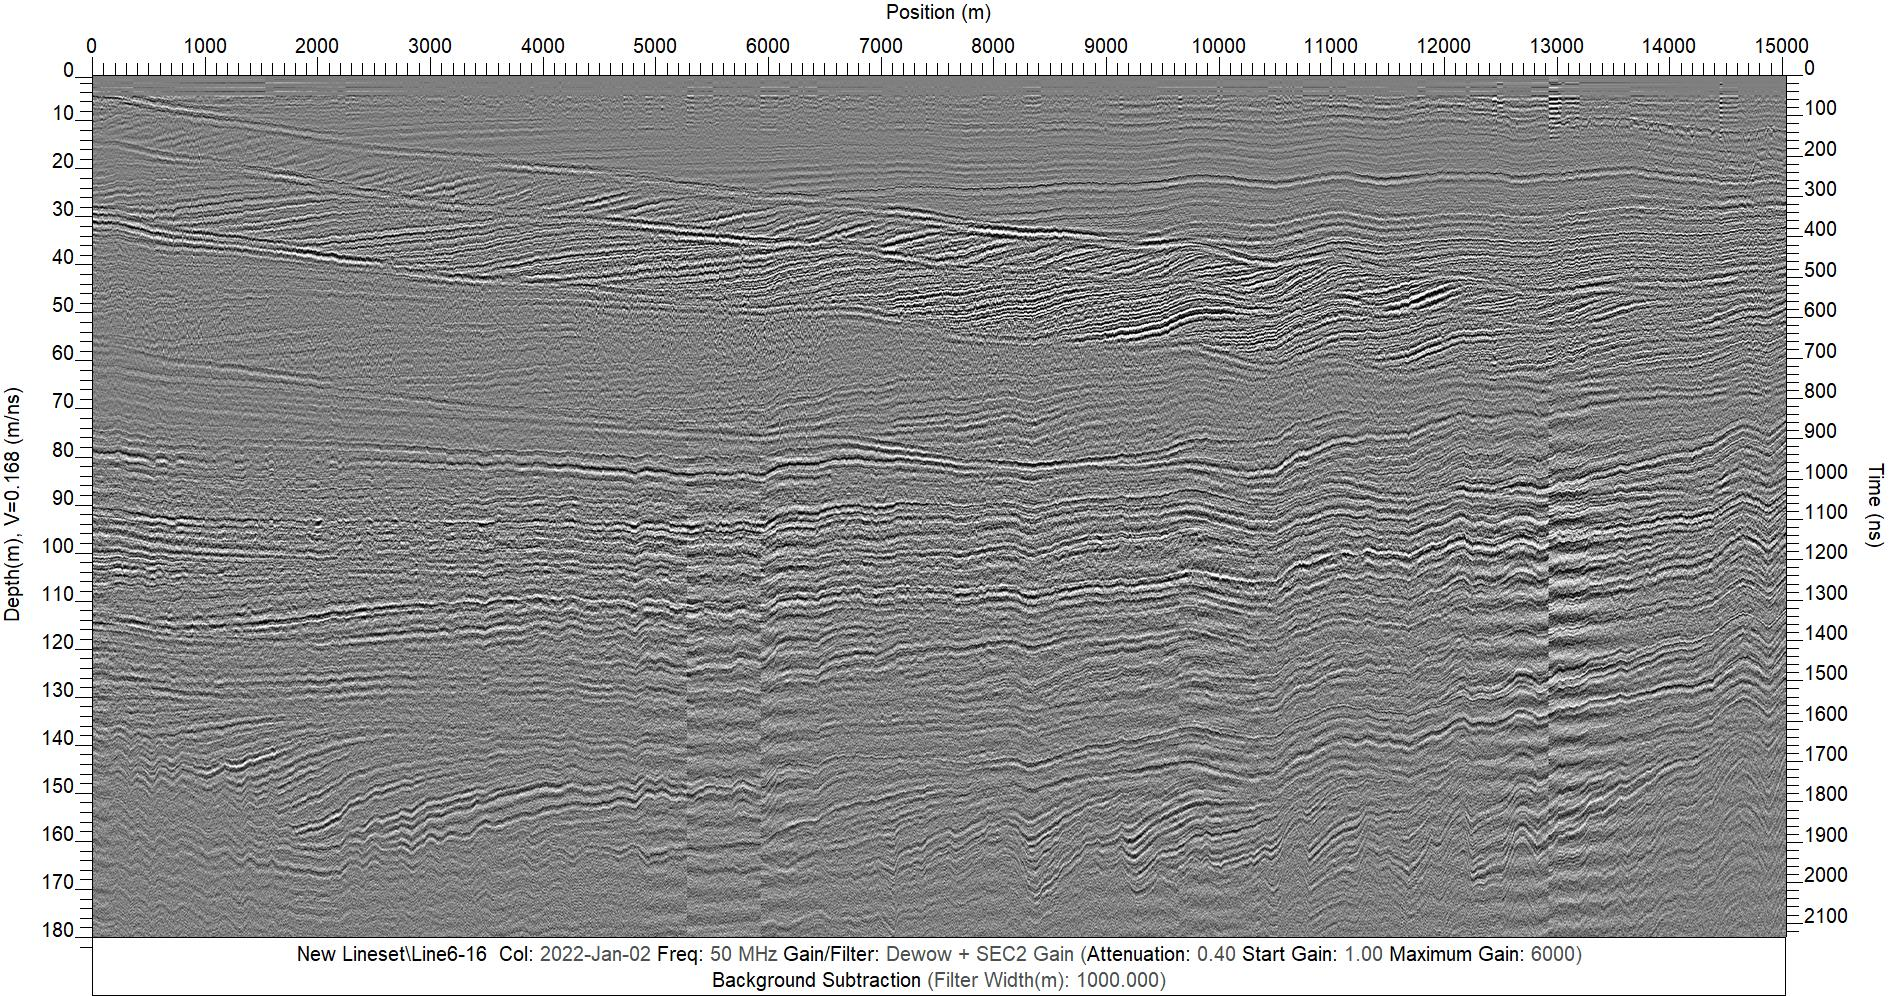
\includegraphics[width=\textwidth]{Figures/PulseEkko/Line6-16-greyr.jpg}
\caption{Cross-cutting internal reflection horizons close to the ice shelf surface (measured with a 50 MHz antennae) detected in the northern part of the coarse ice shelf survey.}.
\label{fig_IRH2}
\end{figure}

%% ******************************************************
%% ******************************************************
\pagebreak
%% ******************************************************
%% ******************************************************
\section{SPM: Data example, field picture, system setup and site specifics}
\label{SecSPM}
\textbf{This section is written by Reza Ershadi}
(\href{mailto:mohammadreza.ershadi@uni-tuebingen.de}{\color{blue}{Email Me}})\\

The SPM points were measured in two different ways.
\begin{itemize}
\item We drove to the point by
Hilux. We set up the system (ApRES and antenna) every time at each point. In
this method, the antennas were directly on the snow surface (fig. \ref{fig_SPM_surface}). The
coordinates and date of the measurements are written in table (\ref{Table_SPM_surface}).
\item We fixed the system (ApRES and antenna) inside the sleds and drove to the points by a
snowmachine (fig. \ref{fig_SPM_sled}). The coordinates and date of the measurements are written in
table (\ref{Table_SPM_sled}).
\end{itemize}
More information on these points is in the following path:\\
..\textbackslash Tex\textbackslash Info\textbackslash RE\_SPM\_Points\_Info.csv\\
..\textbackslash Tex\textbackslash Info\textbackslash RE\_BulletPointReport.txt

\subsection{SPM: Antenna directly on snow surface}
\begin{figure}[H]
	\includegraphics[width=\linewidth]{Figures/SPM_OnSurface.pdf}
	\caption{SPM four antenna (mimo) measurements. Antenna directly on the snow surface.
  The yellow and green rectangles are the tape sign an each antenna. 
  The brown sticks and circles are the bamboo poles.
  The system was positioned in a way that T was always in the South direction.}
	\label{fig_SPM_surface}
\end{figure}

\begin{table}[H]
  \tiny
  \centering
  \rowcolors{2}{gray!25}{white}
  \begin{tabular}[width=\textwidth]{c c c c c c}
    \rowcolor{gray!50}
    Name & Date & Latitude & Longitude & pRES & Note\\
    \hline
    SPM X 04 & 06.12.2021 &  &  & 127 & Unattened mimo test with RTK GPS running \\ 
    SPM A 01 & 06.12.2021 &  &  & 127 & Note \\
    SPM A 04 & 06.12.2021 &  &  & 127 & Note \\
    SPM A 06 & 07.12.2021 & S70 54.6083 & W8 35.0011 & 127 & Note \\
    SPM A 08 & 07.12.2021 & S70 59.6685 & W8 29.5190 & 127 & Note \\
    SPM A 10 & 07.12.2021 & S71 04.8188 & W8 24.1606 & 127 & Note \\
    SPM A 12 & 07.12.2021 & S71 09.9336 & W8 19.5682 & 127 & Note \\
    SPM A 11 & 07.12.2021 & S71 07.3516 & W8 21.8561 & 127 & Note \\
    SPM A 09 & 07.12.2021 & S71 02.2326 & W8 26.9498 & 127 & Note \\
    SPM A 07 & 07.12.2021 & S70 57.1200 & W8 32.0608 & 127 & Note \\
    SPM A 05 & 07.12.2021 & S70 52.1103 & W8 38.0142 & 127 & Note \\
    SPM X 12 & 07.12.2021 & S70 48.5407 & W8 37.3807 & 127 & Note \\
    SPM X 05 & 08.12.2021 & S70 42.1876 & W8 36.2362 & 127 & Note \\
    SPM X 06 & 08.12.2021 & S70 42.9845 & W8 42.2801 & 127 & Note \\
    SPM A 02 & 08.12.2021 & S70 44.6456 & W8 47.2300 & 127 & Note \\
    SPM A 03 & 08.12.2021 & S70 4?.0996 & W8 43.9270 & 127 & Note \\
    SPM X2 13 & 08.12.2021 & S70 49.5042 & W8 44.3598 & 127 & Note \\
    SPM X2 12 & 08.12.2021 & S70 48.6233 & W8 38.4010 & 127 & Note \\
    SPM X3 01 & 01.01.2022 & S71 0.1622 & W7 37.8862 & 127 & Note \\
    SPM X3 02 & 01.01.2022 & S71 0.8448 & W7 44.6390 & 127 & Note \\
    SPM X3 03 & 01.01.2022 & S71 1.0425 & W7 46.5675 & 127 & Note \\
    SPM X3 04 & 01.01.2022 & S71 1.4077 & W7 50.0373 & 127 & Note \\
    SPM X3 05 & 01.01.2022 & S71 1.5366 & W7 52.3067 & 127 & Note \\
    SPM X3 06 & 01.01.2022 & S71 1.6515 & W7 52.5199 & 127 & Note \\
    SPM X3 07 & 01.01.2022 & S71 2.0236 & W7 56.2648 & 127 & Note \\
    SPM X3 08 & 01.01.2022 & S71 2.4512 & W8 0.4169 & 127 & Note \\
    SPM X3 09 & 01.01.2022 & S71 8.2488 & W8 8.3205 & 127 & Note \\
    SPM X3 10 & 01.01.2022 & S71 4.0086 & W8 16.2397 & 127 & Note \\
    SPM A 13 & 01.01.2022 & S71 12.5541 & W8 17.6910 & 127 & Note \\
    SPM A 14 & 01.01.2022 & S71 15.2070 & W8 16.5035 & 127 & Note \\
    SPM A 15 & 01.01.2022 & S71 17.8907 & W8 16.5801 & 127 & Note \\
    SPM A 16 & 01.01.2022 & S71 20.5795 & W8 16.6960 & 127 & Note \\
    SPM A 17 & 01.01.2022 & S71 23.2723 & W8 16.9177 & 127 & Note \\
    SPM A 18 & 01.01.2022 & S71 25.9609 & W8 17.1657 & 127 & Note \\
    SPM A 25 & 04.01.2022 & S71 43.5428 & W8 35.8674 & 128 & Note \\
    \hline
  \end{tabular}
  \caption{SPM on surface info}
  \label{Table_SPM_surface}
\end{table}

\begin{figure}[H]
	\includegraphics[width=\linewidth]{Figures/SPM_X_05.png}
	\caption{Data example from SPM\_X\_05 (floating ice - far from the GZ)}
	\label{fig_SPM_X_05}
\end{figure}

\begin{figure}[H]
	\includegraphics[width=\linewidth]{Figures/SPM_A_25.png}
	\caption{Data example from SPM\_A\_25 (grounded ice - very close to the GZ)}
	\label{fig_SPM_A_25}
\end{figure}

\subsection{SPM: Antenna inside the sleds}
\begin{figure}[H]
	\includegraphics[width=\linewidth]{Figures/SPM_OnSled.pdf}
	\caption{SPM four antenna (mimo) measurements. Antenna inside sleds.
  The yellow and green rectangles are the tape sign an each antenna. 
  The brown sticks and circles are the bamboo poles. 
  The system was positioned in a way that T was always in the South direction.}
	\label{fig_SPM_sled}
\end{figure}

\begin{table}[H]
  \tiny
  \centering
  \rowcolors{2}{gray!25}{white}
  \begin{tabular}[width=\textwidth]{c c c c c c}
    \rowcolor{gray!50}
    Name & Date & Latitude & Longitude & pRES & Note\\
    \hline
    SPM X 01 & 10.12.2021 & S70 38.9781 & W8 12.1931 & 127 &  \\
    SPM X2 11 & 11.12.2021 & S70 47.7299 & W8 32.4452 & 127 &  \\
    SPM X2 10 & 11.12.2021 & S70 46.8444 & W8 26.5088 & 127 &  \\
    SPM X2 09 & 11.12.2021 & S70 45.9602 & W8 20.4776 & 127 &  \\
    SPM X 03 & 12.12.2021 & S70 40.5602 & W8 24.2193 & 127 &  \\
    SPM X 02 & 12.12.2021 & S70 39.7987 & W8 17.4478 & 127 &  \\
    SPM X2 01 & 13.12.2021 & S70 43.2433 & W8 2.8528 & ? &  \\
    SPM X2 02 & 13.12.2021 & S70 43.5002 & W8 4.3377 & ? &  \\ 
    SPM X2 03 & 13.12.2021 & ? & ? & ? & double check needed \\
    SPM X2 04 & 13.12.2021 & ? & ? & ? & double check needed \\
    SPM X2 05 & 13.12.2021 & S70 44.145 & W8 8.7386 & ? &  \\
    SPM X2 06 & 13.12.2021 & S70 44.4317 & W8 10.4649 & ? &  \\
    SPM X2 07 & 13.12.2021 & S70 44.7319 & W8 12.5599 & ? &  \\
    SPM X2 08 & 13.12.2021 & S70 45.0474 & W8 14.6026 & ? &  \\
    SPM A 22 & 7.01.2022 & S71 36.3400 & W8 24.1557 & 127 & Same setup as rover in traverse\\
    SPM A 19 & 7.01.2022 & S71 28.6556 & W8 17.4667 & 127 & Same setup as rover in traverse\\
    SPM A 20 & 7.01.2022 & S71 31.3291 & W8 18.3103 & 127 & Same setup as rover in traverse\\
    SPM A 21 & 7.01.2022 & S71 33.8910 & W8 20.5898 & 127 & Same setup as rover in traverse\\
    SPM A 23 & 7.01.2022 & S71 38.7621 & W8 27.8876 & 127 & Same setup as rover in traverse\\
    SPM A 24 & 7.01.2022 & S71 41.1405 & W8 31.9045 & 127 & Same setup as rover in traverse\\
    SPM X4 01 & 08.01.2022 & S71 25.0643 & W8 45.4317 & 127 & Same setup as rover in traverse\\
    SPM X4 02 & 08.01.2022 & S71 54.3048 & W8 43.9249 & 127 & Same setup as rover in traverse\\
    SPM X4 03 & 08.01.2022 & S71 45.5403 & W8 42.3649 & 127 & Same setup as rover in traverse\\
    SPM X4 04 & 08.01.2022 & S71 45.7?64 & W8 40.8149 & 127 & Same setup as rover in traverse\\
    SPM X4 05 & 08.01.2022 & S71 46.0135 & W8 39.2839 & 127 & Same setup as rover in traverse\\
    SPM X4 06 & 08.01.2022 & S71 46.2455 & W8 37.7977 & 127 & Same setup as rover in traverse\\
    SPM X4 07 & 08.01.2022 & S71 46.4827 & W8 36.1669 & 127 & Same setup as rover in traverse\\
    SPM X4 08 & 08.01.2022 & S71 46.7199 & W8 34.6045 & 127 & Same setup as rover in traverse\\
    \hline
  \end{tabular}
  \caption{SPM on sled info}
  \label{Table_SPM_sled}
\end{table}
%% ******************************************************
%% ******************************************************
\pagebreak
%% ******************************************************
%% ******************************************************
\section{MP\_A (profiling)}
\textbf{This section is written by Reza Ershadi}
(\href{mailto:mohammadreza.ershadi@uni-tuebingen.de}{\color{blue}{Email Me}})\\

The purpose here was to measure a 1000 m profile with 1.5 m spacing with all the
antennas positioned in the H direction. The system was directly connected to an
RTK GPS for precise positioning. We had many problems with this profile,
including the RTK signal, constant ApRES disconnection and typical rover
problems. Therefore, we could not finish the 1000 m profile with 1.5 m spacing.
The position of the profile and measured points are stored in our log files.\\

\textcolor{red}{Add detailed information about the 3 metal pieces. (?)}\\

The MP\_A profile has been done with two different methods.
\begin{itemize}
  \item We pulled the whole sled system manually for 100 m with 1.5 m spacing (fig. \ref{fig_MPA_manual}).
  \item We connected the sled system to the rover for a 1000 m profiling with 1.5 m spacing (fig. \ref{fig_MPA_rover})
\end{itemize}

\subsection{Manually pulling the sleds}
\begin{figure}[H]
	\includegraphics[width=\linewidth]{Figures/MPA_manual.pdf}
	\caption{Manually pulling the ApRES and sleds}
	\label{fig_MPA_manual}
\end{figure}

\subsection{Using the rover}
\begin{figure}[H]
	\includegraphics[width=\linewidth]{Figures/MPA_rover.pdf}
	\caption{Pulling the ApRES and sleds using the rover}
	\label{fig_MPA_rover}
\end{figure}
%% ******************************************************
%% ******************************************************
\pagebreak
\section{HF ApRES}
%: Data example, field picture, system setup and profile specifics
\label{SecHFApRES}

\subsection{System Overview}
The HF ApRES is a frequency modulated continuous wave (FMCW) radar with 
a bandwidth of \SI{20}{\mega\hertz} to \SI{40}{\mega\hertz}.  It builds
upon the existing phase-coherent radar architecture of the ApRES\footnote{
  P. Brennan, L. Lok, K. Nicholls and H. Corr, "Phase‐sensitive FMCW radar 
  system for high‐precision Antarctic ice shelf profile monitoring", IET 
  Radar, Sonar \& Navigation, vol. 8, no. 7, pp. 776-786, 2014. Available: 
  10.1049/iet-rsn.2013.0053.
} but uses a modified radio front-end to operate at the reduced bandwidth
described.  In addition to the radar, the HF ApRES makes use of two 'wire-mesh
dipole' antennas - one each for the transmitter and receiver, and a 12V 
\SI{7}{\ampere\hour} lead-acid battery for power.  Both the HF ApRES radar unit 
and  the 'wire-mesh dipole' antennas had not been previously deployed on a 
polar ice shelf.  The objectives for the HF ApRES system were therefore to test
and validate its performance, then conduct a synthetic aperture radar survey of
the ice-ocean interface of the ice shelf.

\subsubsection{System Equipment Listing}
\begin{itemize}
  \item 1x HF ApRES (VAB Issue C and RMB2F in Pelicase)
  \item 2x Wire-Mesh Dipole Antennas
  \item Clusons 12V \SI{7}{\ampere\hour} Lead Acid Battery
  \item 4x Radiall RG213 \SI{5}{\metre} 50$\Omega$ RF Cables (R284C0351044)
  \item 2x Gigatronix LBC400 \SI{25}{\metre} 50$\Omega$ RF Cables (APX2KDP6ZAB40L)
  \item 2x \SI{10}{\deci\bel} RF attenuators
  \item Various RF connectors
  \item Trimble R9s Modular GNSS System (receiver and base station with UHF
  radio link)
  \item Bamboo and 10mm kernmantle rope for towed configuration.
\end{itemize}

\begin{figure}[htbp]
  \centering
  
  \begin{tikzpicture}[font=\sffamily]
    \node[above right, inner sep=0, draw, black, line width=2pt] (img) at (0,0) {
      \includegraphics[width=0.9\textwidth]{Figures/ApRES/Rover/HF/hf-apres-neumayer.jpg}
    };
    \begin{scope}[x={(img.south east)}, y={(img.north west)}]
      
      % Temporary grid
      % \draw[gray,step=0.1] (img.south west) grid (img.north east);
      % End temporary grid
      \contourlength{1pt}
      \node (tx_ant) at (0.16,0.375) {\contour{white}{\bfseries Tx Antenna}};
      \node (rx_ant) at (0.85,0.375) {\contour{white}{\bfseries Rx Antenna}};
      \node (rx_ant) at (0.5,0.5) {\contour{white}{\bfseries HF ApRES}};

      \draw[latex-latex,ucl_red,line width=1pt] (0.25,0.38) -- 
      node[midway,below] {\contour{white}{\bfseries 5-15m (End-End)}} (0.73,0.38);

      \draw[latex-latex,ucl_red,line width=1pt] (0.16,0.6) -- 
      node[midway,above] {\contour{white}{\bfseries 10-20m (Phase Centres)}} (0.85,0.6);
    
    \end{scope}

  \end{tikzpicture}


  \caption{
    Deployed HF ApRES radar positioned in centre of transmit (Tx) and receive
    (Rx) antennas in endfire configuration.
  }
  \label{FigHFApRESNeumayer}
\end{figure}

\subsection{Testing Summary}
Testing was first conducted with the wire-mesh antennas to verify that they 
met the power transfer characteristics predicted through simulation.  Once
verified, a setup with the full HF ApRES system was configured and issues
were found with strong coupling between the transmit and receive antennas.
After further testing, it was found that broadside orientation of the antennas
and increased separation reduced the direct coupling between the antennas 
sufficiently for clean deramped signals to be recorded.


\begin{table}
  \rowcolors{2}{gray!25}{white}
  \begin{tabular}{m{1.5cm} m{2.25cm} m{7cm} >{\raggedright\arraybackslash}m{3cm}}
    \rowcolor{gray!50}
    Date & Frequency & Profile & File-ID\\
    \hline
    27.12.21 & 30 MHz & Testing of antennas and HF ApRES near Neumayer & \textit{Testing.db} \\
    28.12.21 & 30 MHz & (as above) & \textit{Testing.db} \\
    29.12.21 & 30 MHz & (as above) & \textit{Testing.db} \\
    30.12.21 & 30 MHz & (as above) & \textit{Testing.db} \\
    02.01.22 & 30 MHz & Testing of HF ApRES at Camp & \textit{Testing.db} \\
    03.01.22 & 30 MHz & (as above) & \textit{Testing.db} \\
    04.01.22 & 30 MHz & (as above) & \textit{Testing.db} \\
    05.01.22 & 30 MHz & (as above) & \textit{Testing.db} \\
    06.01.22 & 30 MHz & Testing of HF ApRES at Camp and relocate to GL & \textit{Testing.db} \\
    07.01.22 & 30 MHz & Initial measurements of start-stop survey at GL & \textit{Testing.db, StartStop.db} \\
    08.01.22 & 30 MHz & Complete measurement of start-stop survey at GL and attempt kinematic surveys & \textit{Testing.db, StartStop.db} \\
    \hline
  \end{tabular}
  \label{TableHFApRES}
  \caption{Overview of measurements taken with HF ApRES System.  Individual data
  files are described within the \textit{Testing} and \textit{StartStop}
  databases.  Schema for the databases can be found in the Appendix
  \ref{AppendixHFApRESDatabaseSchemata} of this report.} 
\end{table}

\subsubsection*{Wire-Mesh Dipole Antennas}
The wire-mesh dipole antennas were each tested with an SDRKits Vector Network
Analyzer (VNA) which allows for the measurement of the antenna reflection
coefficient ($\Gamma$).  The reflection coefficient is calculated from the
scattering parameters (s-parameters) measured by the VNA, where $S_{11}$ 
refers to the complex phasor ratio between the scattered and incident voltages from
the antenna.  The reflection coefficient can therefore be used to infer the 
ratio of incident power to the antenna which is 'accepted' and sets an upper
bound on the radiation efficiency.  The radiation efficiency of the antenna
is the ratio of incident power to the antenna that is actually radiated
rather than scattered back to the radar, or lost through conduction within the
antenna structure.  Radiation efficiency is difficult to measure in a field 
environment, hence the reflection coefficient is used to determine an upper
bound.

\begin{equation}
  \left|\Gamma\right|_{\texttt{dB}} = 20\log_{10} \left|S_{11}\right|
\end{equation}

The measured reflection coefficient of the wire-mesh dipole antennas from tests
on 28\textsuperscript{th} December is shown in Figure
\ref{FigureWireMeshNeumayer}.  Within the field of antenna engineering, a
reflection coefficient of less than \SI{-10}{\deci\bel} across the desired
signal bandwidth, i.e. greater than 90\% of power accepted by the antenna, is
deemed to be acceptable.  It can be seen that during initial tests conducted
\SI{500}{\metre} south-west of Neumayer Station the antennas have a measured
$\left|S_{11}\right|_{\textrm{dB}}$ of less than \SI{-10}{\deci\bel} across the
desired signal bandwidth of \SI{20}{\mega\hertz} to \SI{40}{\mega\hertz}.
Discussion regarding the antenna orientation can be below.

\paragraph*{Note:} After transport of the antennas from Neumayer III to the
grounding line camp, it was found that one of the centre-pin conductors on the
antenna arms had become loose, likely due to a dry solder joint.

\begin{figure}[htbp]
  \centering
  \includegraphics[width=\textwidth]{Figures/ApRES/Rover/HF/antenna_comparison_s11.png}
  \caption{
    Measured power reflection coefficient for HF wire-mesh dipole antennas, 
    positioned approximately \SI{500}{\metre} south-west of Neumayer Station.
  }
  \label{FigureWireMeshNeumayer}
\end{figure}

\subsubsection*{HF ApRES Radar}
Figure \ref{FigureHFApRESNoReceiveAntenna} shows a meaured test profile at
Neumayer Station where it was discovered that the receiving antenna of the HF
ApRES radar was disconnected.  A radar echo from is visible at approximately 
\SI{250}{\metre} depth, which corresponds with the expected thickness of the ice
shefl in the vicinity of the station.  The working explaination for the clear,
high signal-to-noise ratio (SNR) echo from the ice-shelf base with no receiving
antenna is that the echo is received by the transmitting antenna and coupled via
the 5V power rail to the receive RF path.  Other coupling paths, such as from the
transmit antenna to the mixer input or via a reflection from the disconnected
receiver port, are ruled out because they would not exibit the \SI{10}{\decibel}
step change in power with the value of the receive attenuator.  An alternative
explanation to be explored through simulation is that the received signal is
coupled through the coaxial cable connected to the receive port, acting as a
poorly matched whip antenna.

\begin{figure}[h]
  \centering
  \input{Figures/ApRES/Rover/HF/apres_updated_rf_chain.tikz}
  \caption{
    System level diagram of the RMB2F radar, showing the signal path from the
    direct digital synthetiser (DDS) to the transmit output, receiver input and
    ouput deramped FMCW signal.}
  \label{FigureHFApRESRadarArchitecture}
\end{figure}

\apresdoc
{2021-12-28-213752.dat}
{Neumayer III}
{Antennas aligned E-W, no receive antenna connected but clear return from
ice-shelf base and double bounce.}
{2021-12-28 21:37:53.000}
{6,6,6,6}
{30,20,10,0}
{1.000}
{20}
{40}
{4}
{40}
{10}
{127}
{12.129}
{FigureHFApRESNoReceiveAntenna}

Reconnecting the receiver antenna, as shown in Figure
\ref{FigureHFApRESReconnectedAntenna} results in sigificant distortion visible
in the time-domain FMCW voltage signal, matched with the reduced SNR seen in the
range-power profile.  Overall power is increased relative to Figure
\ref{FigureHFApRESNoReceiveAntenna}, which gives confidence that the antenna was
not connected and has been successfully reconnected in the second dataset.  The
distortion is characteristic of 'clipping' where the recorded signal exceeds the
voltage range of the analogue-to-digital converter and the output is
subsequently 'clipped' to be within this range.  The evidence of clipping, at
low frequencies corresponding to short range echoes suggests that the direct
coulping between the antennas is higher than experienced from a previous
deployment of the HF ApRES radar on an Alpine glacier. 

\apresdoc
{2021-12-28-214326.dat}
{Neumayer III}
{Antennas aligned E-W, receive antenna reconnected and low-frequency (i.e. near
range) distortion present in signal resulting in reduced signal-to-noise ratio.}
{2021-12-28 21:43:26.000}
{6,6,6,6}
{30,20,10,0}
{1.000}
{20}
{40}
{4}
{40}
{10}
{127}
{12.158}
{FigureHFApRESReconnectedAntenna}

\paragraph*{Antenna orientation} was shown to influence coupling between
the transmit and receive antennas and the presence of high-power low frequency
signals in the deramped FMCW voltage signal.  Broadside refers to the antennas
positioned such that their phase centres are in line with the survey direction
and their longest axes are orthogonal to the survey direction.  Endfire refers
to the antennas positioned such that their longest axes are parallel to the
survey direction.  Experiemnts repeated at Neumayer Station (Figures
\ref{FigureHFApRESEndfireNeumayer} and \ref{FigureHFApRESBroadsideNeumayer}) and
the grounding line camp (Figures \ref{FigureHFApRESEndfireGroundingLine} and
\ref{FigureHFApRESBroadsideGroundingLine}) show that thwne antennas are aligned
in a 'broadside' configuration they exhibit reduced near-range coupling compared
to antennas separated by the same distance in an 'endfire' configuration.  The
HF ApRES was then reconfigured to be operated with the SubZero rover in a
broadside configuration, with an increased separation between the transmit and
receive antennas of \SI{40}{\metre}.

\begin{figure}[htbp]
  \centering
  \begin{tikzpicture}[font=\sffamily]
    \node[above right, inner sep=0, draw, black, line width=2pt] (img) at (0,0) {
      \includegraphics[width=0.8\textwidth]{Figures/ApRES/Rover/HF/hf-apres-subzero.jpg}
    };
    \begin{scope}[x={(img.south east)}, y={(img.north west)}]
      
      % Temporary grid
      % \draw[gray,step=0.1] (img.south west) grid (img.north east);
      % End temporary grid

      \contourlength{1pt}
      \node[anchor=east] at (0.33, 0.8) {\contour{white}{ UHF control radio}};
      \node[anchor=east] at (0.31, 0.6) {\contour{white}{Backup GPS}};
      \node[anchor=south] at (0.42, 0.63) {\contour{white}{RTK-GPS}};
      \node[anchor=west] at (0.87, 0.73) {\contour{white}{Tx}};
      \node[anchor=west] at (0.92, 0.62) {\contour{white}{Rx}};
      \node[anchor=west] at (0.65, 0.52) {\contour{white}{HF ApRES}};
      \node[anchor=south] at (0.24, 0.29) {\contour{white}{IMU}};
      \node[anchor=south] at (0.82, 0.73) {\contour{white}{IMU}};
      \node[anchor=south east] at (0.72,0.65) {\contour{white}{IMU}};

      % Draw distance labels
      \draw[latex-latex, line width=0.5pt, ucl_red] (0.81,0.72) -- 
        node[midway,above,anchor=south east,inner sep=1pt,ucl_red] {\contour{white}{40m}} (0.73,0.645);
      \draw[latex-latex, line width=0.5pt, ucl_red] (0.72,0.63) -- 
        node[midway,above,anchor=south east,inner sep=1pt,ucl_red] {\contour{white}{10m}} (0.652,0.552);
      \draw[latex-latex, line width=0.5pt, ucl_red] (0.6,0.5) --
        node[midway,above,ucl_red] {\contour{white}{10m}} (0.45,0.4);
      % \draw[ucl_red, line width=1pt] (0.76, 0.4) rectangle (0.83, 0.8);
      % \node[ucl_red, anchor=south] at (0.79, 0.8) {\contour{white}{\scriptsize 10dB Atten.}};

    \end{scope}
  \end{tikzpicture}
  \caption{
    SubZero rover and HF ApRES configuration used for start-stop and kinematic
    synthetic aperture radar acquisitions at groundling line.
  }
  \label{FigureHFApRESSubZeroConfiguration}
\end{figure}

\apresdoc
{2021-12-29-215659.dat}
{Neumayer III,500m W of Station}
{\textbf{Antenna Orientation: Endfire, Neumayer}. No additional attenuations. Antennas rotated so they are aligned N-S and cables N-S.  Similar to above but with noise in upper layers. 14m separation.  Cables 'smooth' in line with antennas.  Reduced power code to 0.}
{2021-12-29 21:58:31.000}
{6,6,6,6}
{30,20,10,0}
{1.000}
{20}
{40}
{4}
{4}
{1}
{0}
{12.266}
{FigureHFApRESEndfireNeumayer}

\apresdoc{2021-12-29-220442.dat}
{Neumayer III,500m W of Station}
{\textbf{Antenna Orientation: Broadside, Neumayer}. No additional attenuations. Antennas rotated so they are aligned E-W but Tx at N and Rx at S.  Similar to above but with noise in upper layers. 14m separation.  Cables 'smooth' in line with antennas.  Reduced power code to 0.}
{2021-12-29 22:04:45.000}
{6,6,6,6}
{30,20,10,0}
{1.000}
{20}
{40}
{4}
{4}
{1}
{0}
{12.258}
{FigureHFApRESBroadsideNeumayer}

\apresdoc{2022-01-05-174254.dat}
{Grounding Line Camp}
{\textbf{Antenna Orientation: Endfire, Grounding Line}. Additional attenuator 10dB Rx, 0dB Tx.  Cable length Tx 25m, Rx 25m and separate antennas to maximum length (30m).  Antennas return to endfire.  Clipping across all AF settings.  No clear basal return.}
{2022-01-05 17:43:31.000}
{-14,-4,6}
{0,0,0}
{1.000}
{20}
{40}
{3}
{120}
{40}
{127}
{12.238}
{FigureHFApRESEndfireGroundingLine}

\apresdoc{2022-01-05-171029.dat}
{Grounding Line Camp}
{\textbf{Antenna Orientation: Broadside, Grounding Line}. Additional attenuator 10dB Rx, 0dB Tx.  Increase Tx cable to 25m (Rx 5m) and separate antennas to maximum length (30m).  Antennas rotated broadside.  Bed clearer (higher SNR)? Some clipping in signal.  Repeated as before - ringing reduced?}
{2022-01-05 17:10:51.000}
{-14,-4,6}
{0,0,0}
{1.000}
{20}
{40}
{3}
{120}
{40}
{127}
{12.238}
{FigureHFApRESBroadsideGroundingLine}
\clearpage

\subsection{Synthetic Aperture Radar Measurements}
The test site chosen for the HF ApRES SAR measurements was selected to coincide
with the series of basal terraces observed in the PulseEKKO data located in the
finely gridded region of Figure \ref{fig:overview}.  The HF ApRES system was
towed into position on 7\textsuperscript{th} January, configured according to
\ref{FigureHFApRESSubZeroConfiguration} and initial testing was conducted,
including the resolution of a software navigation issue with the rover.  Two
modes of measurement were conducted with the HF ApRES: a start-stop profile
where the instrument was repositioned in steps of \SI{1}{\metre} increments
along the desired profile direct, and kinematic profiles where the radar was set
to continuously measure while towed along the profile by the SubZero rover at
speeds of approximately \SI{0.7}{\metre\per\second} to
\SI{1}{\metre\per\second}.  For all measurement modes, the radar was configured
with the parameters listed in Table \ref{TableHFApRESMeasurementParams}.  The 
VV notation for the polarisation is consistent with that of the rover-towed VHF
system, however the precise polarisation response of the wire-mesh dipole
antennas has not been measured.

\begin{table}[h]
  \rowcolors{2}{gray!25}{white}
  \centering\begin{tabular}{l c r l}
    \hline
    \rowcolor{gray!50}
    Parameter & Symbol & \multicolumn{2}{c}{Value} \\
    \hline
    Centre Frequency & $f_c$ & 30 & \si{\mega\hertz} \\
    Bandwidth & $B$ & 20 & \si{\mega\hertz} \\
    Pulse Duration & $T$ & 1 & \si{\second} \\
    Transmit Power & $P_T$ & 0.1 & \si{\watt} \\
    AF Gain & $G_{AF}$ & 6 & \si{\deci\bel} \\
    RF Attenuation & $A_{RF}$ & 10 & \si{\deci\bel} \\
    RF Atten. (External) & $A_{RFExt}$ & 10 &  \si{\deci\bel} \\
    Antenna Separation & $S_{Ant}$ & 40 & \si{\metre} \\
    Rover Separation & $S_{Rov}$ & 10 & \si{\metre} \\
    Polarisation & - & VV & - \\
    \hline
    
  \end{tabular}
  \caption{Radar configuration parameters common to both the start-stop and
  kinematic the HF ApRES SAR measurements}
  \label{TableHFApRESMeasurementParams}
\end{table}

\subsubsection{Start-Stop Measurement}
On the 7\textsuperscript{th} January, \SI{192}{\metre} of the intended profile
was covered .  The rover was left in position overnight and the profile was
resumed to cover the remaining \SI{710}{\metre} over approximately 5 hours,
including aapproximately one hour of cumulative downtime. The Trimble R9s base
station was set up approximately \SI{40}{\metre} away from the profile at its
centre.  The RINEX files generated by the GNSS receivers at the base station and
on the rover were processed using the Canadian Spatial Reference System Precise
Point Positioning service\footnote{Full details can be found in
\texttt{Raw/RTKGPS/ApRES/Rover/HF/processing\_notes.md}} and are shown in Figure 
\ref{FigureHFApRESGNSS}.  There are tidal and ice flow components present in the
raw position data.  The ice velocity ($v$) is assumed constant along the length
of the profile from analysis of the \SI{120}{\metre} composite ITS\_LIVE data
for 2020.  The tidal components of the measured elevation were analysed using
the Tidal Fitting Toolbox \footnote{\url{https://uk.mathworks.com/matlabcentral/fileexchange/19099-tidal-fitting-toolbox}}
but have not yet been validated with external data.  It is assumed that the
tidal components are also locally invariant and therefore the relative position
of the rover to the base is initially found through subtraction of the base
station coordinates from the rover coordinates. Phase and power of raw data is 
shown in Figure \ref{FigureHFApRESRaw}.

\begin{figure}[h!]
  \centering 
  \includegraphics{../../Doc/ApRES/Rover/HF/StartStop/StartStopRawData.png}
  \caption{Phase and power of raw, unprocessed ApRES data collected along the
  profile.}
  \label{FigureHFApRESRaw}
\end{figure}

Initial SAR processing of the dataset was performed using an interpolated 
$\textrm{sinc}$ routine using the MATLAB\copyright~ ApRESProcessor library\footnote{
\url{https://github.com/jonodhawkins/apresprocessor}} with a constant velocity
travel-time model using a dielectric permittivity for ice of $3.15$.  Antenna
positions were modelled to be \SI{50}{\metre} and \SI{10}{\metre} behind the
rover, in the direction of the image plane, as per the system setup indicated in
Figure \ref{FigureHFApRESSubZeroConfiguration}. For the
intial pass, bursts with low signal to noise ratios compared to the mean of the
dataset were excluded however further passes will select individual chirps from
these bursts to maximise the number of radar locations at which the
backprojection is performed.  Results of the backprojection in power and phase
are shown in Figure \ref{FigureHFApRESBackprojection}.

\begin{figure}[h]
  \centering 
  \includegraphics{../../Doc/ApRES/Rover/HF/StartStop/StartStopInitialInterp.png}
  \caption{Phase and power of initial backprojected (SAR processed) image from
  the HF ApRES towed by the SubZero rover.  The coordinate system for the image
  is relative polar stereographic to the Trimble GPS base station.  Pixel
  resolution is \SI{4}{\metre}.}
  \label{FigureHFApRESBackprojection}
\end{figure}

\begin{figure}[h!]
  \centering 
  \includegraphics{../../Doc/ApRES/Rover/HF/StartStop/StartStopRTKPositions.png}
  \includegraphics{../../Doc/ApRES/Rover/HF/StartStop/StartStopRoverPositions.png}
  \caption{Precise point positioned GPS outputs from Canadian Spatial Reference
  System for rover and base station.  Gray highlighted areas show periods of rover
  operation.  Second plot shows derived relative position of rover to base 
  station, mitigating tidal flexure of ice shelf and positional drift from ice 
  flow.}
  \label{FigureHFApRESGNSS}
\end{figure}

\subsubsection{Kinematic Measurement}
The kinematic measurements were made after the start and stop measurements along
the same profile to provide a comparative dataset and explore the use of the
ApRES radar as a mobile SAR.  Processing of the data is underway and not yet
included in this report.

\clearpage

\pagebreak
%% ******************************************************
%% ******************************************************
\section{cApRES}
\label{SeccApRES}
\textbf{RE,JH}\\

\begin{table}[H]
  \small
  \centering
  \rowcolors{2}{gray!25}{white}
  \begin{tabular}[width=\textwidth]{c c c c c c}
    \rowcolor{gray!50}
    Name & Date & Latitude & Longitude & pRES & Note\\
    \hline
    cApRES & 10.01.2022& S71 36.9565 & W8 25.9803 & 127 & Buried\\
    \hline
  \end{tabular}
  \caption{cApRES}
  \label{Table_cApRES}
\end{table}

The initial cApRES setup used cables of different lengths.  One-way travel times
for the cables were measured using an SDRKits VNA in time-domain reflectometer
(TDR) and network analyser (VNA) modes.  The `Yellow' cable was removed from the
initial setup and replaced with the `Double Earth' cable to reduce the
difference in cable travel time.  Final antenna cabling and assignments are
listed in Table \ref{TablecApRESCables}. 
The ApRES was configured to measure every \SI{3}{\hour}, alternating between 
mono-polarised (HH) and quad-polarised (HH, HV, VH, VV) measurements.  The RF
attenuator was set to \SI{23}{\decibel} and the AF gain was set to 
\SI{-14}{\decibel}.  The chirp settings are the default values with a sweep of
\SI{200}{\mega\hertz} to \SI{400}{\mega\hertz} over a period of \SI{1}{\second}.

\begin{figure}[H]
  \centering
  \includegraphics[width=0.6\linewidth]{Figures/CApRES/CApRES_Setup.jpg}
  \caption{Photograph of cApRES Measurement Setup on 9\textsuperscript{th}
  January 2022, prior to burying of ApRES and replacement of `Yellow' coaxial
  cable.}
  \label{FigCApRESSetupImage}
\end{figure}

\begin{figure}[H]
  \includegraphics[width=\linewidth]{Figures/cApRES.pdf}
  \caption{Diagram of cApRES Measurement Setup}
  \label{fig_cApRES}
\end{figure}

\begin{table}[H]
  \centering
  \rowcolors{2}{gray!25}{white}
  \begin{tabular}[width=\textwidth]{l c c c c}
    \hline
    \rowcolor{gray!50}
    Cable Colour & Antenna ID & ApRES Port & Polarisation & 1-Way Travel Time (ns) \\
    \hline
    Blue Earth & 315 & Rx 2 & V & 26.69 \\
    Double Earth & 309 & Rx 1 & H & 26.69 \\
    Red & 308 & Tx 1 & H & - \\
    Green & 307 & Tx 2 & V  & - \\
    Yellow & Unused & - & - & 22.31 \\
    \hline
  \end{tabular}
  \caption{Antenna and cabling configuration for cApRES measurement setup.  
  One-way travel times for the `Red` and `Green' cables were not measured.}
  \label{TablecApRESCables}
\end{table}

\begin{figure}[h]
  \includegraphics[width=\textwidth]{Figures/CApRES/test_burst_2022-01-10_184911.png}
  \caption{Example data from the cApRES measurement setup taken on 10\textsuperscript{th}
  January 2022 at 18:49:11 UTC.}
\end{figure}
\clearpage
%% ******************************************************
%% ******************************************************
\pagebreak
%% ******************************************************
%% ******************************************************
\section{Rover-ApRES: Data example, field picture, system setup and site specifics}
\label{SecRoverApRES}
\textbf{This section is written by Reza Ershadi}
(\href{mailto:mohammadreza.ershadi@uni-tuebingen.de}{\color{blue}{Email Me}})\\
\begin{figure}[H]
	\includegraphics[width=\linewidth]{Figures/Traverse_Rover_Profiling.pdf}
	\caption{Antenna setup for ApRES profiling with the rover and sleds}
	\label{fig_rover}
\end{figure}
\begin{figure}[H]
	\includegraphics[width=\linewidth]{Figures/Rover_ApRES_Results.png}
	\caption{Radar power obtained by the rover-sled profiling system.}
	\label{fig_rover_res}
\end{figure}

%\ProtocolTable{Setup PulseEkko Radar}{N/A}{PulseEkko 50 MHz}{N/A}{I. Koch}{N/A}

% \begin{minipage}[t]{\textwidth}
%
% \end{minipage}


\clearpage
\appendix
\section{HF ApRES Database Schemata}
\label{AppendixHFApRESDatabaseSchemata}

\newcommand{\sqlspectable}[2]{
    \renewcommand{\arraystretch}{1.5}
    \rowcolors{2}{gray!10}{white}
    \begin{longtable}{l l >{\raggedright}p{3cm} >{\raggedright\arraybackslash}p{4cm}}
        \caption{#2} \\
        \hline
        \rowcolor{gray!50}
        \textbf{Fieldname} & \textbf{Datatype} & \textbf{Parameters} & \textbf{Description}\\
        \hline
        \endhead
        \hline
        \endfoot
        #1
    \end{longtable}
}

\subsection{Table `\texttt{measurements}'} 
\sqlspectable{
    %
    measurement\_id & INTEGER & PRIMARY KEY & 
    Unique identifier for each file. \\
    %
    filename & TEXT & NOT NULL & 
    Filename without path. \\
    %
    path & TEXT & UNIQUE NOT NULL&
    Path to file in UNIX form, relative to top-level project root. \\
    %
    name & TEXT & - &
    The name associated with the measurement, used to group sets of 
    measurements together. \\
    %
    timestamp & TEXT & UNIQUE ASC NOT NULL &
    \texttt{YYYY-mm-dd HH:MM:SS.fff} formatted timestamp according to
    time and date the measurement was taken. \\
    %
    valid & INTEGER & NOT NULL DEFAULT 0 &
    Boolean indicator of whether file is valid. Assumes invalid by 
    default. \\
    %
    base\_visible & INTEGER & NOT NULL DEFAULT 0 & 
    Boolean indicator of whether basal reflector is visible in range data. \\
    %
    base\_range\_min & REAL & NOT NULL DEFAULT -1 & 
    Minimum range (in steps of 50m) at which basal reflector can be found. \\
    %
    base\_range\_max & REAL & NOT NULL DEFAULT -1 & 
    Maximum range (in steps of 50m) at which basal reflector can be found. \\
    %
    location & TEXT & - & 
    Measurement location name. \\
    % 
    comments & TEXT & - &
    Description and comments for measurement if relevant. \\
    % 
    latitude & REAL & - &
    Latitude of measurement location if known. \\
    %
    longitude & REAL & - & 
    Longitude of measurement location if known. \\
    %
    elevation & REAL & - & 
    Elevation of measurement location if known (referenced to WGS84). \\
    %
    tags & TEXT & - & 
    Annotation tags (i.e. \texttt{bad\_chirps}, \texttt{gps\_type}, ...). \\
}
{Specification for \texttt{measurements} table.}

\newpage

\subsection{Table `\texttt{apres\_metadata}'}
The fields \texttt{id} and \texttt{burst\_id} make a unique pair to ensure
that each burst within a \texttt{*.dat} file is only represented once.

\sqlspectable{
    %
    id & INTEGER & PRIMARY KEY & 
    Unique identifier for metadata.  Distinct from \texttt{measurement\_id}
    in that each \texttt{*.dat} file can have multiple bursts.\\
    %
    burst\_id & INTEGER & NOT NULL &
    Identifies the burst within a \texttt{*.dat} the metadata represents.\\
    %
    measurement\_id & INTEGER & NOT NULL & 
    Identifies the file record where the metadata originates from. \\
    %
    % header\_index & INTEGER & NOT NULL DEFAULT 0 &
    % Indicates the byte at which to start reading the header \\
    % % 
    % burst\_index & INTEGER & NOT NULL & 
    % Indicates the byte at which to start reading the data associated with the burst \\
    %
    \hline
    \multicolumn{4}{c}{\textit{ApRES Specific Metadata}} \\
    \hline
    %
    timestamp & TEXT & NOT NULL & 
    \texttt{YYYY-mm-dd HH:MM:SS.fff} formatted timestamp as logged in
    \texttt{*.dat} file. \\
    %
    n\_attenuators & INTEGER & NOT NULL CHECK(\textgreater 0, \textless 5) & 
    Number of attenuator settings used. \\
    %
    n\_chirps & INTEGER & NOT NULL CHECK(\textgreater 0) & 
    Total number of individual chirps in file. \\
    %
    n\_subbursts & INTEGER & NOT NULL CHECK(\textgreater 0) &
    Number of sub-bursts (repeats) of the burst configuration. \\
    %
    period & REAL & NOT NULL CHECK(\textgreater 0) & 
    Chirp period in seconds. \\
    %
    f\_lower & REAL & NOT NULL CHECK($\ge$ 0) &
    Lower bound of chirp ramp in Hertz. \\
    %
    f\_upper & REAL & NOT NULL CHECK($\ge$ 0) & 
    Upper bound of chirp ramp in Hertz. \\
    %
    af\_gain & TEXT & NOT NULL &
    Comma separated values indicating AF gain settings. \\
    %
    rf\_attenuator & TEXT & NOT NULL & 
    Comma separated values indicating RF attenuator settings. \\
    %
    f\_sampling & REAL & NOT NULL CHECK(\textgreater 0) & 
    Sampling frequency. \\
    % 
    tx\_antenna & TEXT & NOT NULL &
    Transmit antenna selection in comma separated value format. \\
    % 
    rx\_antenna & TEXT & NOT NULL &
    Receive antenna selection in comma separated value format. \\
    % 
    power\_code & INTEGER & - &
    DDS output current power code, if available (dependent on firmware).\\
    %
    battery\_voltage & REAL & - &
    Battery voltage, if available. \\
    %
    temperature\_1 & REAL & - &
    Measured board temperature from sensor 1. \\
    %
    temperature\_2 & REAL & - & 
    Measured board temperature from sensor 2. \\
    %
    rmb\_issue & TEXT & - & 
    RMB issue number if available. \\
    % 
    vab\_issue & TEXT & - & 
    VAB issue number if available. \\
    %
    venom\_issue & TEXT & - &
    Venom issue number if available. \\
    %
    software\_issue & TEXT & - & 
    VAB firmware issue number if available. \\
}{
    Specification for \texttt{apres\_metadata} table.
}

\end{document}

    © 2022 GitHub, Inc.

    Terms
    Privacy
    Security
    Status
    Docs
    Contact GitHub
    Pricing
    API
    Training
    Blog
    About

